\chapter{Background Knowledge and Related Work}
\label{sec:background}

This chapter provides an overview of the key concepts and relevant research for this thesis. The goal is to integrate the proposed approaches into the broader context of existing work and show how they contribute to the current state of research.

\section{Embeddings}
\label{sec:background:embeddings}
Embeddings form the foundation of many modern \ac{nlp} systems by providing a mathematical representation of words, texts or other concepts in a continuous vector space, as illustrated in Figure~\ref{fig:embeddings}. These representations capture semantic relationships, enabling machines to better understand and process human language. This section provides an overview of the evolution of embedding techniques, from early static word vectors to more recent context-aware models. Additionally, it emphasizes the importance of embeddings in a variety of \ac{nlp} applications.

\begin{figure}[ht]
  \begin{center}
    % source: https://www.cs.cmu.edu/~dst/WordEmbeddingDemo/tutorial.html
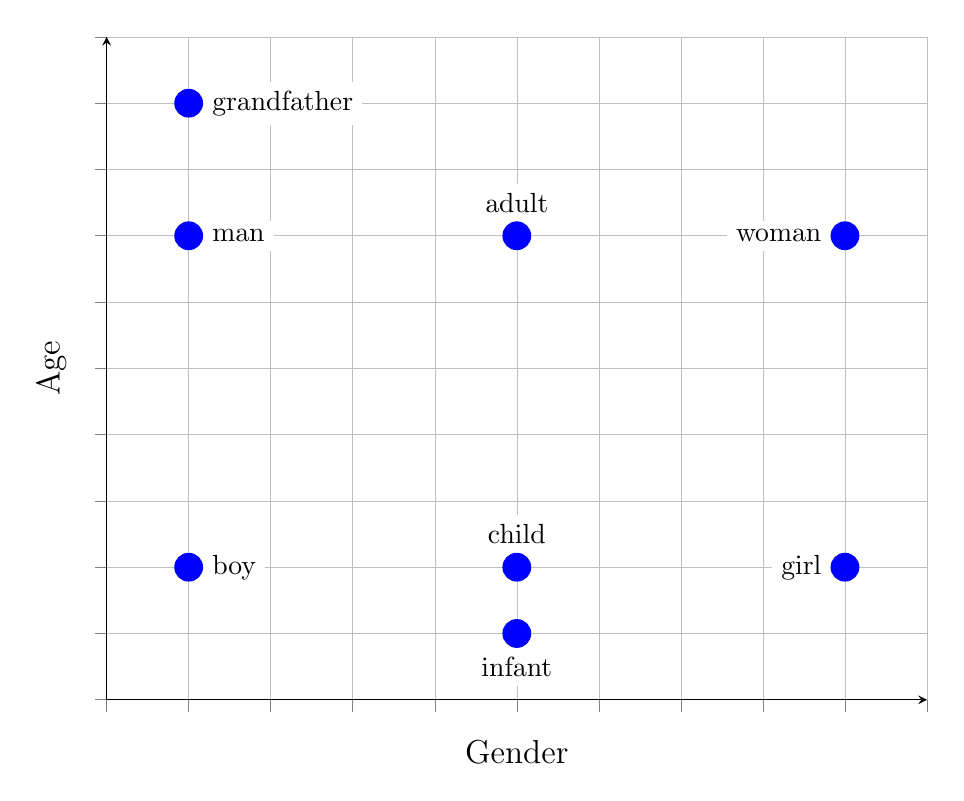
\begin{tikzpicture}
  \begin{axis}[
      width=12cm, height=10cm,
      xlabel={Gender}, ylabel={Age},
      xmin=0, xmax=10, ymin=0, ymax=10,
      xtick={0,1,...,10}, ytick={0,1,...,10},
      xticklabel={\empty}, yticklabel={\empty},
      grid=both,
      grid style={line width=.1pt, draw=gray!30},
      major grid style={line width=.2pt,draw=gray!50},
      axis lines=left,
      tick align=outside,
      enlargelimits=false,
      label style={font=\large},
      title style={font=\LARGE, yshift=1em},
      every tick label/.append style={font=\small},
    ]

    % Plot the points
    \addplot[
      only marks,
      mark=*,
      mark size=5pt,
      blue,
    ] coordinates {
        (1,9)   % grandfather
        (1,7)   % man
        (1,2)   % boy
        (5,7)   % adult
        (5,2)   % child
        (5,1)   % infant
        (9,7)   % woman
        (9,2)   % girl
      };

    % Add labels
    \node[fill=white, anchor=west, xshift=5pt, font=\normalsize] at (axis cs:1,9)  {grandfather};
    \node[fill=white, anchor=west, xshift=5pt, font=\normalsize] at (axis cs:1,7)  {man};
    \node[fill=white, anchor=west, xshift=5pt, font=\normalsize] at (axis cs:1,2)  {boy};
    \node[fill=white, anchor=south, yshift=5pt, font=\normalsize] at (axis cs:5,7)  {adult};
    \node[fill=white, anchor=south, yshift=5pt, font=\normalsize] at (axis cs:5,2)  {child};
    \node[fill=white, anchor=north, yshift=-5pt, font=\normalsize] at (axis cs:5,1)  {infant};
    \node[fill=white, anchor=east, xshift=-5pt, font=\normalsize] at (axis cs:9,7)  {woman};
    \node[fill=white, anchor=east, xshift=-5pt, font=\normalsize] at (axis cs:9,2)  {girl};
  \end{axis}
\end{tikzpicture}
  \end{center}
  \caption{TODO:}
  \label{fig:embeddings} % TODO: reference
\end{figure}

Early models for word representation focused on learning fixed vectors for each word, resulting in what are known as static word embeddings. These embeddings assign the same vector to a word regardless of the context in which it appears. Well-known examples of such approaches include Word2Vec (\cite{mikolovEfficientEstimationWord2013}) and GloVe (\cite{penningtonGloveGlobalVectors2014}), both of which capture semantic similarities based on word co-occurrence statistics in large text corpora.

Although static word embeddings are computationally efficient and useful in many scenarios, they are unable to account for variations in meaning across different contexts. This limitation has led to the development of contextual word embeddings, which are context-dependent. One early example is ELMo (\cite{petersDeepContextualizedWord2018}), which uses bidirectional \ac{lstm} networks to generate embeddings sensitive to surrounding words in a sentence.

More recent approaches use transformer-based architectures. Models such as BERT (\cite{devlin-etal-2019-bert}) generate deep contextual embeddings using self-attention mechanisms to model relationships between words within a given context. Contextual information is crucial because it enables models to disambiguate polysemous words. For example, the word \enquote{bank} can refer to a financial institution or the side of a river, and only contextual clues can determine the intended meaning.

These contextual embeddings have substantially improved performance across a wide variety of \ac{nlp} tasks, including question answering, named entity recognition, and machine translation. As a result, they have become essential components of modern \ac{nlp} pipelines.

\section{Stylistic Investigations}
\label{sec:background:styleInvestigations}
% TODO: write a little more about the proxy tasks; what are they, what are examples, why are they necessary
% TODO: example for learned style embedding method with citation
The objective of Stylistic Investigations is to identify an author's unique writing style independent of the content being expressed. Modern neural approaches often accomplish this by learning dense vector representations, or style embeddings, through proxy tasks. These tasks include style transfer, authorship attribution or verification, and group membership detection. Proxy tasks enable models to learn stylistic features without explicit style annotations. This is important because annotating large amounts of data is very difficult and time-consuming.

However, one drawback of learned style embeddings is that it is difficult to ensure that the representations are truly independent of the content, as noted by \citet{wegmannSameAuthorJust2022}. This complicates their application in new domains where the content may differ. Additionally, such embeddings tend to be uninterpretable, reducing their transparency and limiting their usefulness in downstream tasks.

Some approaches aim to produce interpretable embeddings to address these issues. Notable examples include the work by \citet{patelLearningInterpretableStyle2023}, who propose a method for learning attribute-based representations, and \citet{alshomaryLatentSpaceInterpretation2024}, who focus on interpreting latent embeddings. This thesis builds on and extends this line of research by proposing a new method for learning interpretable style embeddings that incorporate knowledge-related dimensions.

Other, more classical methods for stylistic analysis take a different approach. They work by manually selecting interpretable features such as the frequency of function words, syntactic structures, or punctuation counts. These features are extracted using comprehensible algorithms and can be used to construct explainable classifiers, although they may lack the nuance and representational capacity of neural embeddings.
\citet{okulskaStyloMetrixOpensourceMultilingual2023} presented Stylometrix as an example of recent work in this area. It generates interpretable style vectors based on a curated set of features. Another example is StyloAI, which was developed \citet{oparaStyloAIDistinguishingAIgenerated2024a} and extracts 31 stylometric features to identify AI-generated texts using a Random Forest classifier.

The main advantages of feature-based approaches are the relevance and quality of the extracted features. However, these methods have several drawbacks. First, they require manual feature selection, which limits the range of stylistic attributes that can be captured. Additionally, these methods cannot incorporate more abstract attributes requiring a deeper understanding of the text, such as the knowledge-related features employed in this thesis.

\section{Large Language Models}
\label{sec:background:llm}

\Acfp{llm} are large-scale neural networks with billions of parameters. These models are pre-trained on massive text corpora and can perform tasks that require advanced language understanding and generation (\cite{minaeeLargeLanguageModels2025}).
\acp{llm} have brought significant advancements to the field of \acl{nlp}, achieving state-of-the-art performance in a broad range of applications. These include text generation, translation, and question answering, among many others.

The transformer architecture, introduced by \citet{NIPS2017_3f5ee243} in the seminal paper \enquote{Attention Is All You Need}, is the foundation of most modern \acp{llm}. Unlike earlier models, which relied on recurrence or convolution, the transformer architecture uses self-attention mechanisms to weigh the relevance of each word in the input sequence relative to the others. This design supports parallel processing, thereby improving training efficiency and scalability.

As shown in Figure~\ref{fig:transformerArchitecture}, the transformer follows an encoder-decoder architecture. The encoder processes the input sequence and produces a continuous representation. Then, the decoder generates the output sequence based on the encoder's output and previous outputs. There are encoder-only models, such as embedding models, that produce a representation of the input text. There are also decoder-only models that predict subsequent tokens based on previous outputs or a prompt.

This thesis will employ encoder-only models to create interpretable attribute embeddings. Decoder-only \acp{llm} will be used for the task of text generation.

\begin{figure}[ht]
  \begin{center}
    \input{figures/tikz/transformer-architecture.tex}
  \end{center}
  \caption{TODO:} % TODO: mention source (attention is all you need); explain layers
  % source: https://www.cs.cmu.edu/~dst/WordEmbeddingDemo/tutorial.html
  \label{fig:transformerArchitecture}
\end{figure}

\section{Steering of Large Language Models}
\label{sec:background:llm:steering}

Although \acp{llm} are highly effective at generating coherent and fluent text, it is often desirable to guide the generated text to follow specific constraints or stylistic forms. It is also essential to prevent models from generating toxic or inappropriate content. Several steering methods have been developed to address these challenges.

One widely used method is \textbf{prompt engineering}, which involves steering the model by modifying the input prompt provided during inference. The key advantage of this approach is that it does not require any model training (\cite{schulhoffPromptReportSystematic2024}).

There are several variations of prompt engineering. One important type involves changing the system prompt, which is particularly relevant in chat-based \acp{llm}. A system prompt defines how a model behaves and what tone it uses throughout a conversation. Although it is hidden from the user, the system prompt can influence the model to adopt a specific persona, adhere to formatting rules, or follow safety guidelines. For instance, the system prompt can instruct the model to act as a helpful tutor or avoid discussing certain topics. This steering technique will be evaluated in this thesis.

Another variant of prompt engineering is few-shot prompting. With this approach, the prompt contains instructions for the task and a few examples of correct task completions. These examples allow the model to generalize to similar tasks by recognizing patterns.

% chain-of-thought prompting by Wei et al., 2022 % TODO: include this?

\textbf{Fine-tuning} is a more resource-intensive method of steering that involves updating the parameters of the model using task-specific data. Although fine-tuning can yield strong performance, it is often too expensive for \acp{llm} due to their size. Furthermore, using a different fine-tuned model for each task can be inefficient and impractical.

To mitigate these issues, parameter-efficient fine-tuning methods have been developed. These methods freeze the pre-trained model weights and only train a small number of additional parameters. One such method is prefix tuning (\cite{liPrefixtuningOptimizingContinuous2021}), where a learned vector (prefix) is prepended to the model input. This method achieves competitive performance while training only \SI{0.1}{\percent} of the model's parameters. Another example is LoRA (\cite{huLoRALowrankAdaptation2021}), which introduces trainable low-rank matrices into the model while keeping the original weights fixed. LoRA reduces the number of trainable parameters by a factor of \num{10000} without compromising performance.

% \textbf{Reinforcement Learning from Human Feedback (RLHF)} % TODO: include this?

A recent alternative to these methods is \textbf{activation steering}, which directly alters the hidden states of an \acs{llm} during inference to guide its output. These hidden states are generally accessed at the end of each transformer layer. Modern \acp{llm} typically consist of between \num{20} and \num{100} such layers, with deeper layers typically encoding more abstract and sophisticated concepts (\cite{bogdanEmergentEffectsScaling2025}).

Activation steering involves identifying and extracting the hidden states that correspond to specific concepts in a single forward pass. These extracted vectors, known as steering vectors, are added to the internal states of the model during inference to guide the generation process in the desired direction (\cite{konenStyleVectorsSteering2024,turnerActivationAdditionSteering2024,subramaniExtractingLatentSteering2022}).
